% \documentclass[../main.tex]{subfiles}

% \begin{document}
\section{Introduction}
\label{introduction}



% First para -> motivation (why are you doing this work, what did you find missing in the society)
% 2+3 para -> macro view -> zoom in (cite a few papers) (these are the existing tools, pros, cons, define bio index with applications (sociatal/computatinal), key generation
% 3rd para -> problem statement (small intro)
% 
\subsection{Background}
Biometrics, also known as biometric recognition, is a process of automated recognition of any individual on the basis of some of their behavioral and/or physiological trait. \cite{Jain2004}
We, as humans, have used a person's face, gait, or voice to distinguish them from other people around us or recognize them for thousands of years. In the late 19th century, a need for an automated recognition system using biometrics, particularly fingerprints, arose for identifying criminals and storing them in a database.
Some examples of biometrics are DNA, fingerprint, face, gait, voice, hand or ear geometry, hand or finger vein infrared thermograph, iris, retina, keystroke, odor, palmprint, and signature/handwriting and can be seen in figure \ref{fig:bio_ex} \cite{Jain2004}.
\begin{figure}[!ht]
    \centering 
    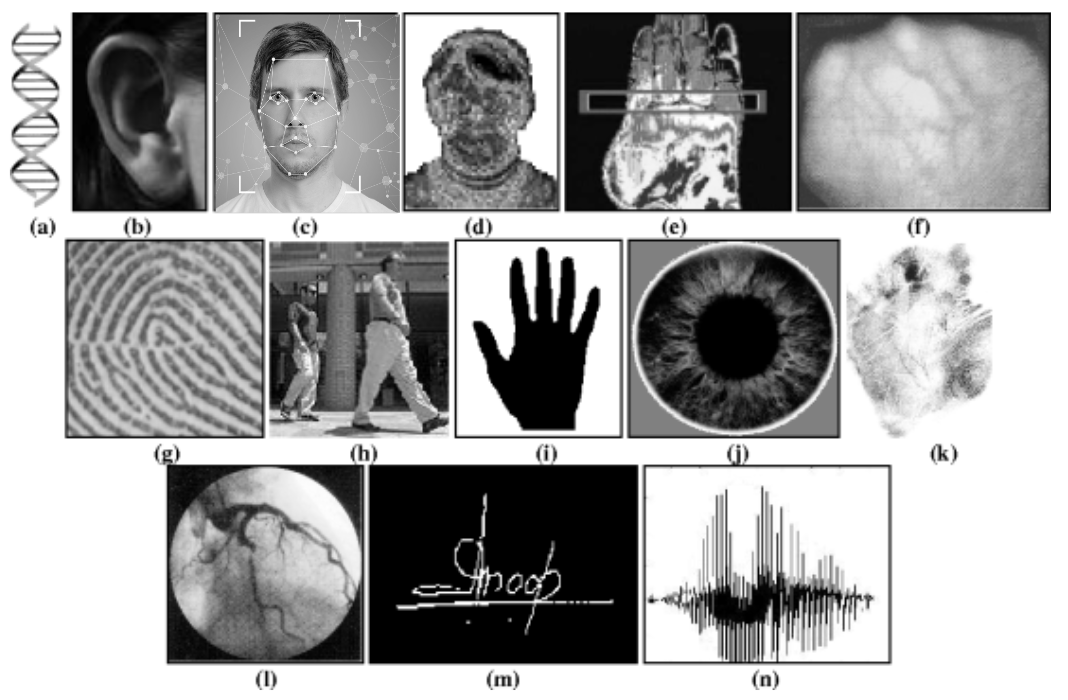
\includegraphics[width=0.45\textwidth]{images/Examples of biometric characteristics.png}
    \caption{Examples of biometric characteristics: (a) DNA profiling, (b) ear shape, (c) facial features, (d) facial thermograph, (e) hand thermograph, (f) hand vein profile, (g) fingerprints, (h) gait, (i) hand geometry, (j) iris, (k) palmprint, (l) retina scans, (m) signature, and (n) voice.}
    \label{fig:bio_ex}
\end{figure}


% What are the traits/features of a person that qualify as a biometric? \cite{Unar2014}
% \begin{itemize}
%     \item \textit{Universality}: present in every person
%     \item \textit{Distinctiveness}: two people having the given trait should have sufficient difference
%     \item \textit{Collectability}: the trait should be fairly easy to collect and quantify/feature extraction
%     \item \textit{Permanence}: over time, the trait should not change (eg. as a person ages)
%     \item \textit{Performance}: availability of resources constraints in data collection, and the guarantee of high accuracy when matching
%     \item \textit{Acceptability}: the willingness of people to submit the trait and privacy risks involved 
%     \item \textit{Circumvention}: prone to imitation or fraudulent attempts to mimic the trait 
% \end{itemize}
% Table \ref{table:bio_trait_comp} lists a number of biometric traits and gives a brief comarision of each biometric a score based on the above mentioned factors. No biometric is perfect/optimal as it always lacks one of the requirements (e.g. accuracy, cost, practicality). Fingerprints are widely used as a biometric because they offer many advantages over other biometrics mainly in terms of ease of acquisition, temporal invariance and uniqueness among different subjects.\cite{Jain1997}
% \begin{table}[!ht]
%     % \scriptsize
%     % \renewcommand{\arraystretch}{2}
%     \centering
%     \caption{Comparison of Biometric Traits \cite{Jain2004} (High=100, Medium=50, Low=0)}
%     % \renewcommand{\arraystretch}{10}
%     \begin{center}
%     \begin{tabular}{|l|l|l|l|l|l|l|l|l|}
%     \hline
%         % Biometric Trait & \rot{Universality} & \rot{Distinctiveness} & \rot{Permanence} & \rot{Collectability} & \rot{Performance} & \rot{Acceptability} & \rot{Circumvention} & \rot{Average} \\ \hline
%         \textbf{Biometric Trait} & \rot{Universality} & \rot{Distinctiveness} & \rot{Permanence} & \rot{Collectability} & \rot{Performance} & \rot{Acceptability} & \rot{Circumvention} & \rot{Average} \\ \hline
%         Fingerprint & 50 & 100 & 100 & 50 & 100 & 50 & 50 & 71.4 \\ \hline
%         Palmprint & 50 & 100 & 100 & 50 & 100 & 50 & 50 & 71.4 \\ \hline
%         Face & 100 & 0 & 50 & 100 & 0 & 100 & 100 & 64.3 \\ \hline
%         Ear & 50 & 50 & 100 & 50 & 50 & 100 & 50 & 64.3 \\ \hline
%         Facial thermogram & 100 & 100 & 0 & 100 & 50 & 100 & 0 & 64.3 \\ \hline
%         Iris & 100 & 100 & 100 & 50 & 100 & 0 & 0 & 64.3 \\ \hline
%         DNA & 100 & 100 & 100 & 0 & 100 & 0 & 0 & 57.1 \\ \hline
%         Hand geometry & 50 & 50 & 50 & 100 & 50 & 50 & 50 & 57.1 \\ \hline
%         Odor & 100 & 100 & 100 & 0 & 0 & 50 & 0 & 50.0 \\ \hline
%         Retina & 100 & 100 & 50 & 0 & 100 & 0 & 0 & 50.0 \\ \hline
%         Gait & 50 & 0 & 0 & 100 & 0 & 100 & 50 & 42.9 \\ \hline
%         Hand vein & 50 & 50 & 50 & 50 & 50 & 50 & 0 & 42.9 \\ \hline
%         Signature & 0 & 0 & 0 & 100 & 0 & 100 & 100 & 42.9 \\ \hline
%         Voice & 50 & 0 & 0 & 50 & 0 & 100 & 100 & 42.9 \\ \hline
%         Keystroke & 0 & 0 & 0 & 50 & 0 & 50 & 50 & 21.4 \\ \hline
%     \end{tabular}
% \end{center}
%     \label{table:bio_trait_comp}
% \end{table}

% Furthermore, Biometric traits can also be classified into many modalities. They most common ones are shown in Figure \ref{fig:bio_class}

% \begin{figure}
%     \centering
%     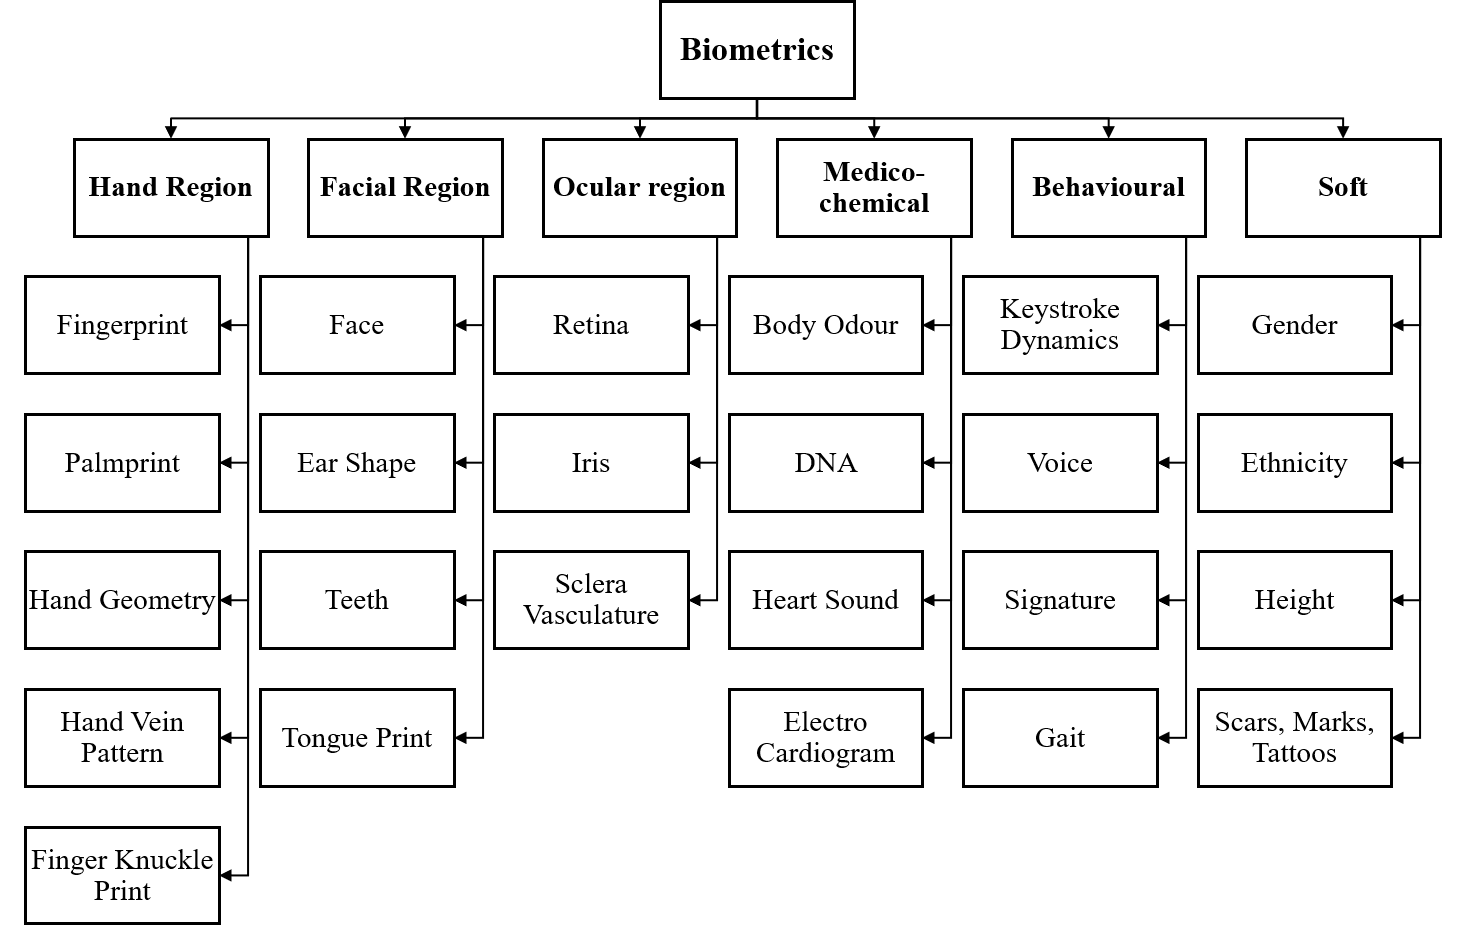
\includegraphics[width=0.75\textwidth]{images/Classification of biometric modalities.png}
%     \caption{Classification of biometric modalities \cite{Unar2014}}
%     \label{fig:bio_class}
% \end{figure}


\subsection{Biometric Authentication System}
A biometric authentication system is a type of pattern recognition system. It can recognize/authenticate a person by
determining whether some behavioral characteristic and/or a specific physiological
possessed by that person is authentic.\cite{Maltoni2003}

Essentially, a biometric system uses acquired biometric data of an individual, extracts numerical features from it, and compares the feature set to that of another person/ or a template set in a database. 
Broadly we can classify biometric systems based on one of two operation modes.
\begin{itemize}
    \item Verification: one-to-one matching, checks if a given biometric matches an existing enrollment. (returns True/False)
    \item Identification: one-to-many matching, recognizes/retries information using an input biometric over a set of existing enrollments. (returns the record or similar linked information)
\end{itemize}

% A biometric system can be subdivided into five subsystems given below and shown in Figure \ref{fig:bio_sys_block}.
% \begin{itemize}
%     \item \textit{Data collection:} Use of sensor or camera to acquire image/snapshot of trait
%     \item \textit{Transmission:} Compression of collected data and transmission to data storage and signal processing module
%     \item \textit{Data storage:} Storage of information in a meaningful manner and template generation for the user
%     \item \textit{Signal processing:} Feature extraction by image processing techniques and pattern matching operations
%     \item \textit{Decision systems:} Identification or Verification of an input using matching scores
% \end{itemize}



\begin{figure}[!ht]
    \centering 
    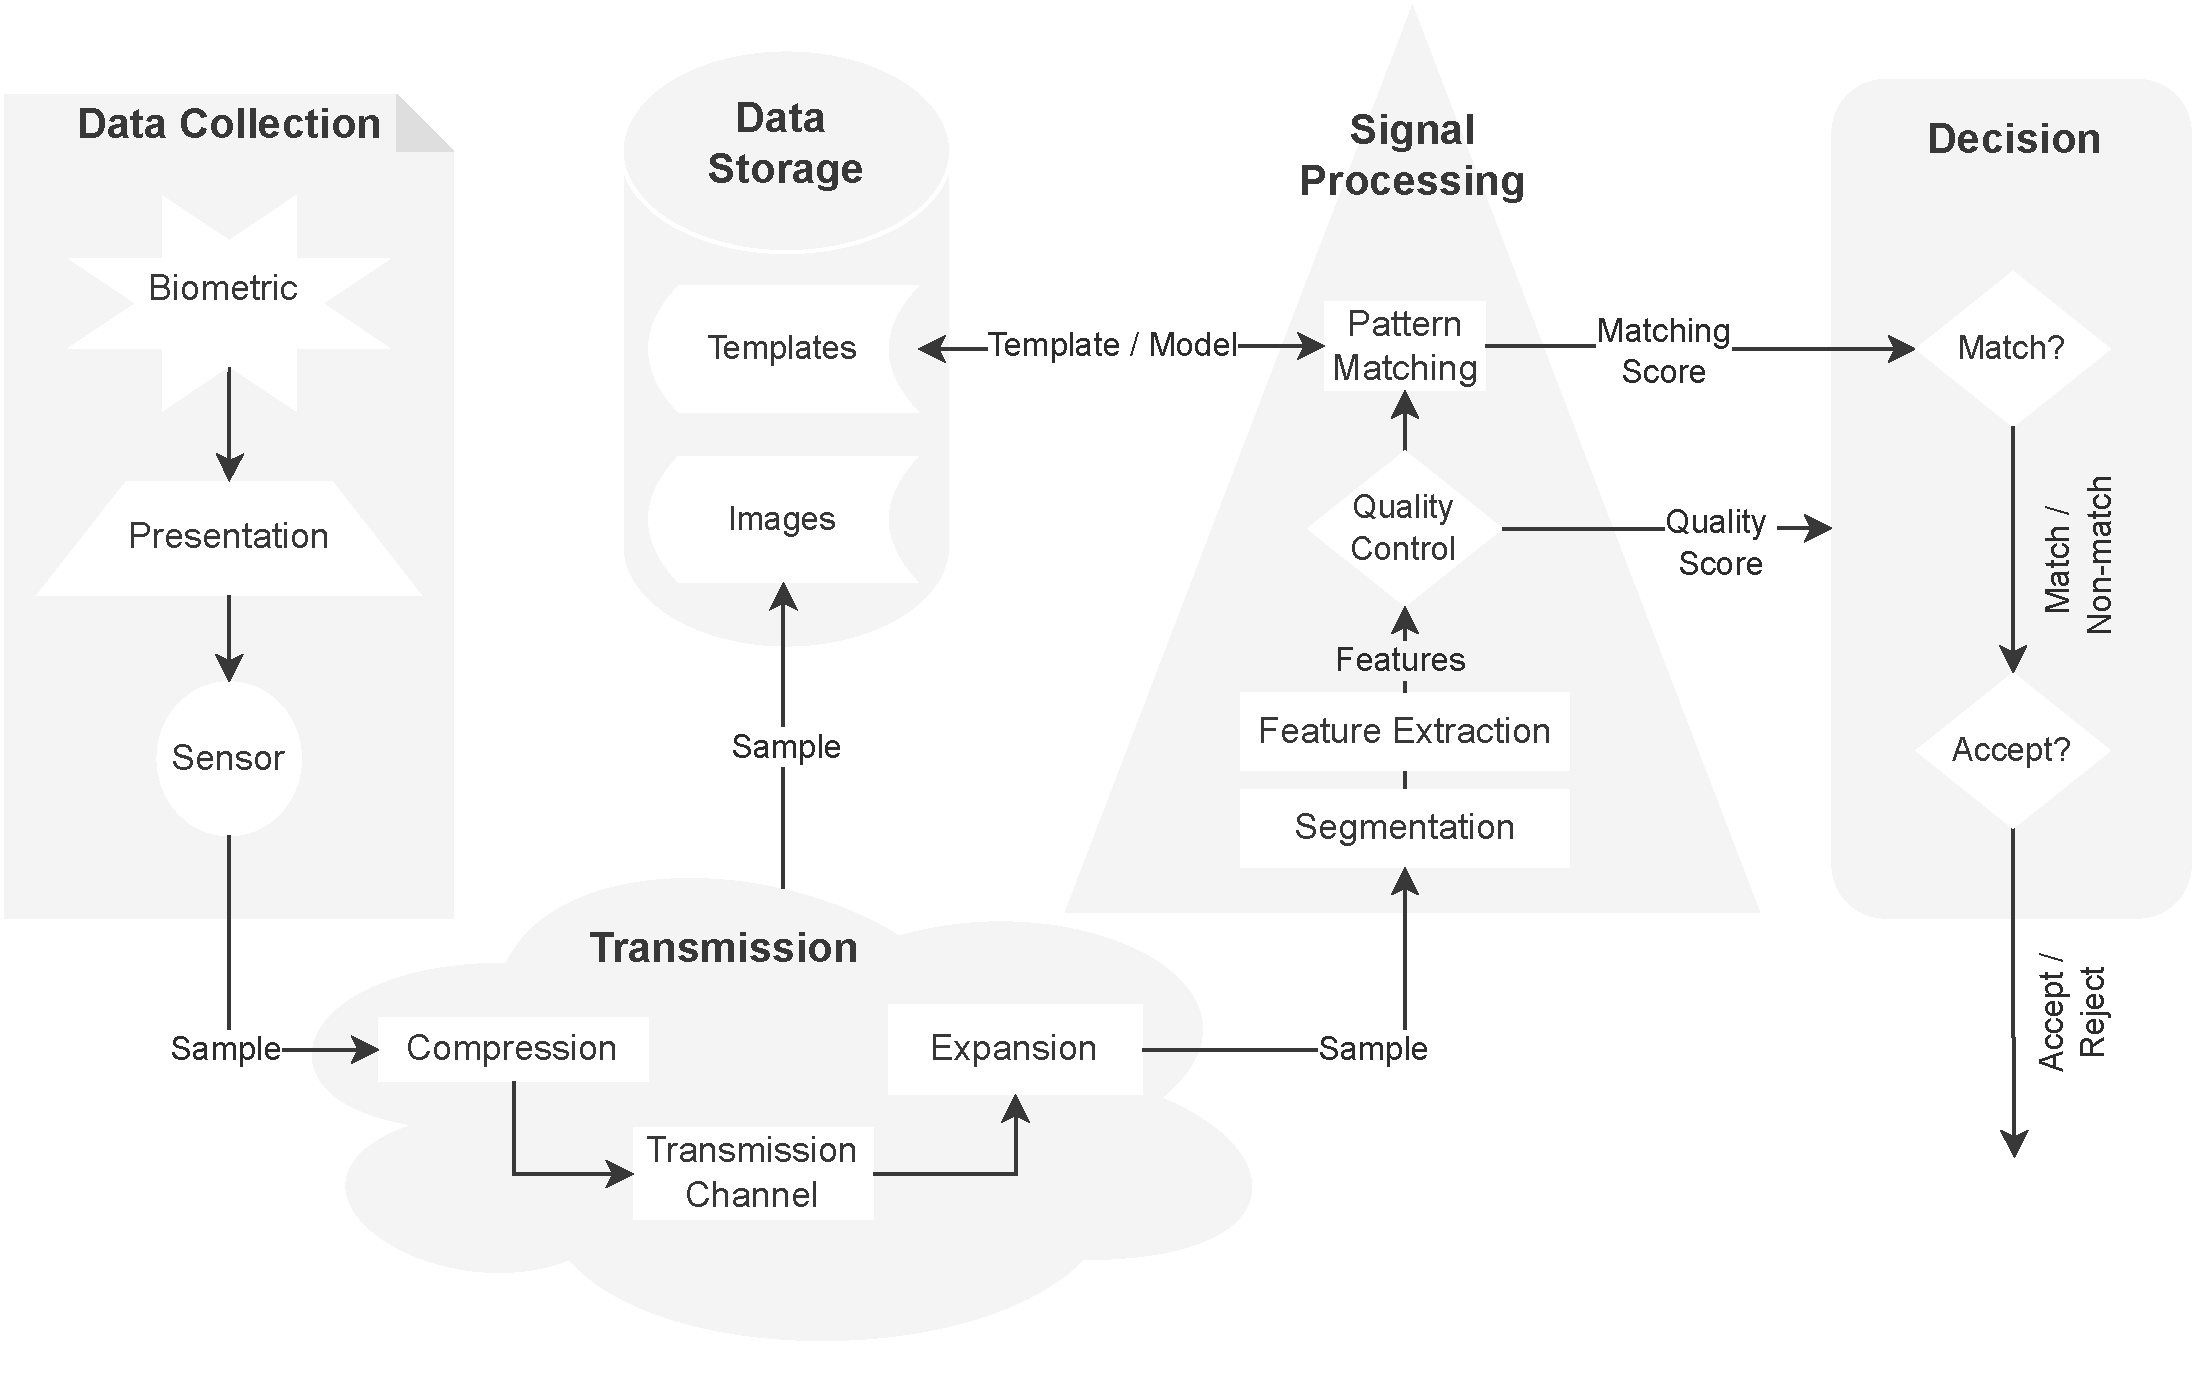
\includegraphics[width=0.55\textwidth]{images/Block diagram of a generic biometric system.png}
    \caption{Block Diagram of a generic biometric system along with its subsystems \cite{Leniski2003}}
    \label{fig:bio_sys_block}
\end{figure}

Figure \ref{fig:bio_sys_block} shows that the first step in any biometric system is the acquisition of biometric data from the users of that system. The acquired data is stored is transmitted in a compressed manner and stored in a secure location. Various techniques can be used for processing the data. Usually, most systems process the incoming data to store them accordingly. This work will be focused on the data storage and signal processing part.

An interesting corner case for a biometric system is the distinction between identical twins. Several works show that accurate verification of an individual from their twin can be done using their fingerprint \cite{Jain2002}, palmprint \cite{Kong2006}, face \cite{Phillips2011}, as well as multimodal traits \cite{Sun2010}. An intriguing note is that each iris of the same person is unrelated to each other \cite{Wildes1997} just like fingerprints from different fingers of the same person, thus vary between twins as well.

\subsection{Indexing}

The definition of data indexing in simple terms is to re-organize/process data items in a database such that we have a key to data in the database
that helps us to find the location of the item in the memory. In indexing search query is taken as input and the collection of matching records is returned efficiently. This index (key) can be calculated by several techniques such that the searching process 
is as time-efficient and space-efficient as possible. However, there is usually an inverse relationship between time and space complexities when using an index.

Mainly Indexes can be classified into the following types \cite{garcia2008database} and is shown in \ref{fig:index_class}:
\begin{itemize}
    \item \textit{Dense Index:} All the data is sorted based on a unique attribute, also known as the primary key. There exists an index record (that has the key and holds the pointer to the data with the key) for every search key in the data file. This can help to search faster but as a drawback it
needs significantly more space in order to store the index records.
    \item \textit{Sparse Index:} Only some index records pointing to the start of blocks are stored, which are like containers of data. This is to have better space complexity than dense indexing but the search time is slower. Reference to all the keys does not exist. Pointers point 
only to the first key of the block. Thus, it cannot be determined directly from the index if a key is present until the pointer is followed and the block is checked thoroughly.
    \item \textit{Secondary Indexing:} This is a kind of a two-level indexing technique and is used to reduce the mapping size of the first level. Between index 
records and actual data blocks, there exist buckets in between. 
There are indexes on these buckets and these buckets contain pointers to the actual data.
It is kind of a mix of sparse(index on buckets) and dense(buckets to data) indexing to be more efficient.
    \item \textit{Hashing:} A Hash Function maps a key to a bucket in which actual data is stored. Simply put, a query key is passed into the hash function and the output is the pointer to the container where the data is present.
    \item \textit{B-Tree(B+ Tree):} It is a data structure for tree-based indexing. It is constructed in such a way that all leaf nodes contain actual data pointers with 
    key values in them. 
    All leaf nodes are connected like a linked list to support random and sequential access. 
    The non-leaf nodes contain keys and pointers to navigate to the required value. 
    If a non-leaf node has n search keys then, it will have n+1 pointers (a pointer 
    to the left and right of every key). If the query key is less than the search key then the left pointer is used to navigate further otherwise the right pointer is used.
    \item \textit{kd-Tree:} It is a generalization of binary search trees to multidimensional data. 
    In other words, a kd-tree is a space partitioning data structure in a k-dimensional space.
    Similar to a binary tree, a non-leaf node in the kd-tree divides the space into 2 parts.
    Points to the left of this space are represented by the left subtree of that 
    node and points to the right of the space are represented by the right subtree. 
    Each level in the tree goes on dividing the plane into 
    separate planes and each non-leaf node contains the plane/attribute on which the space is divided. 
    Leaf nodes are the blocks with records in the space.
\end{itemize}

\begin{figure}
    \centering
    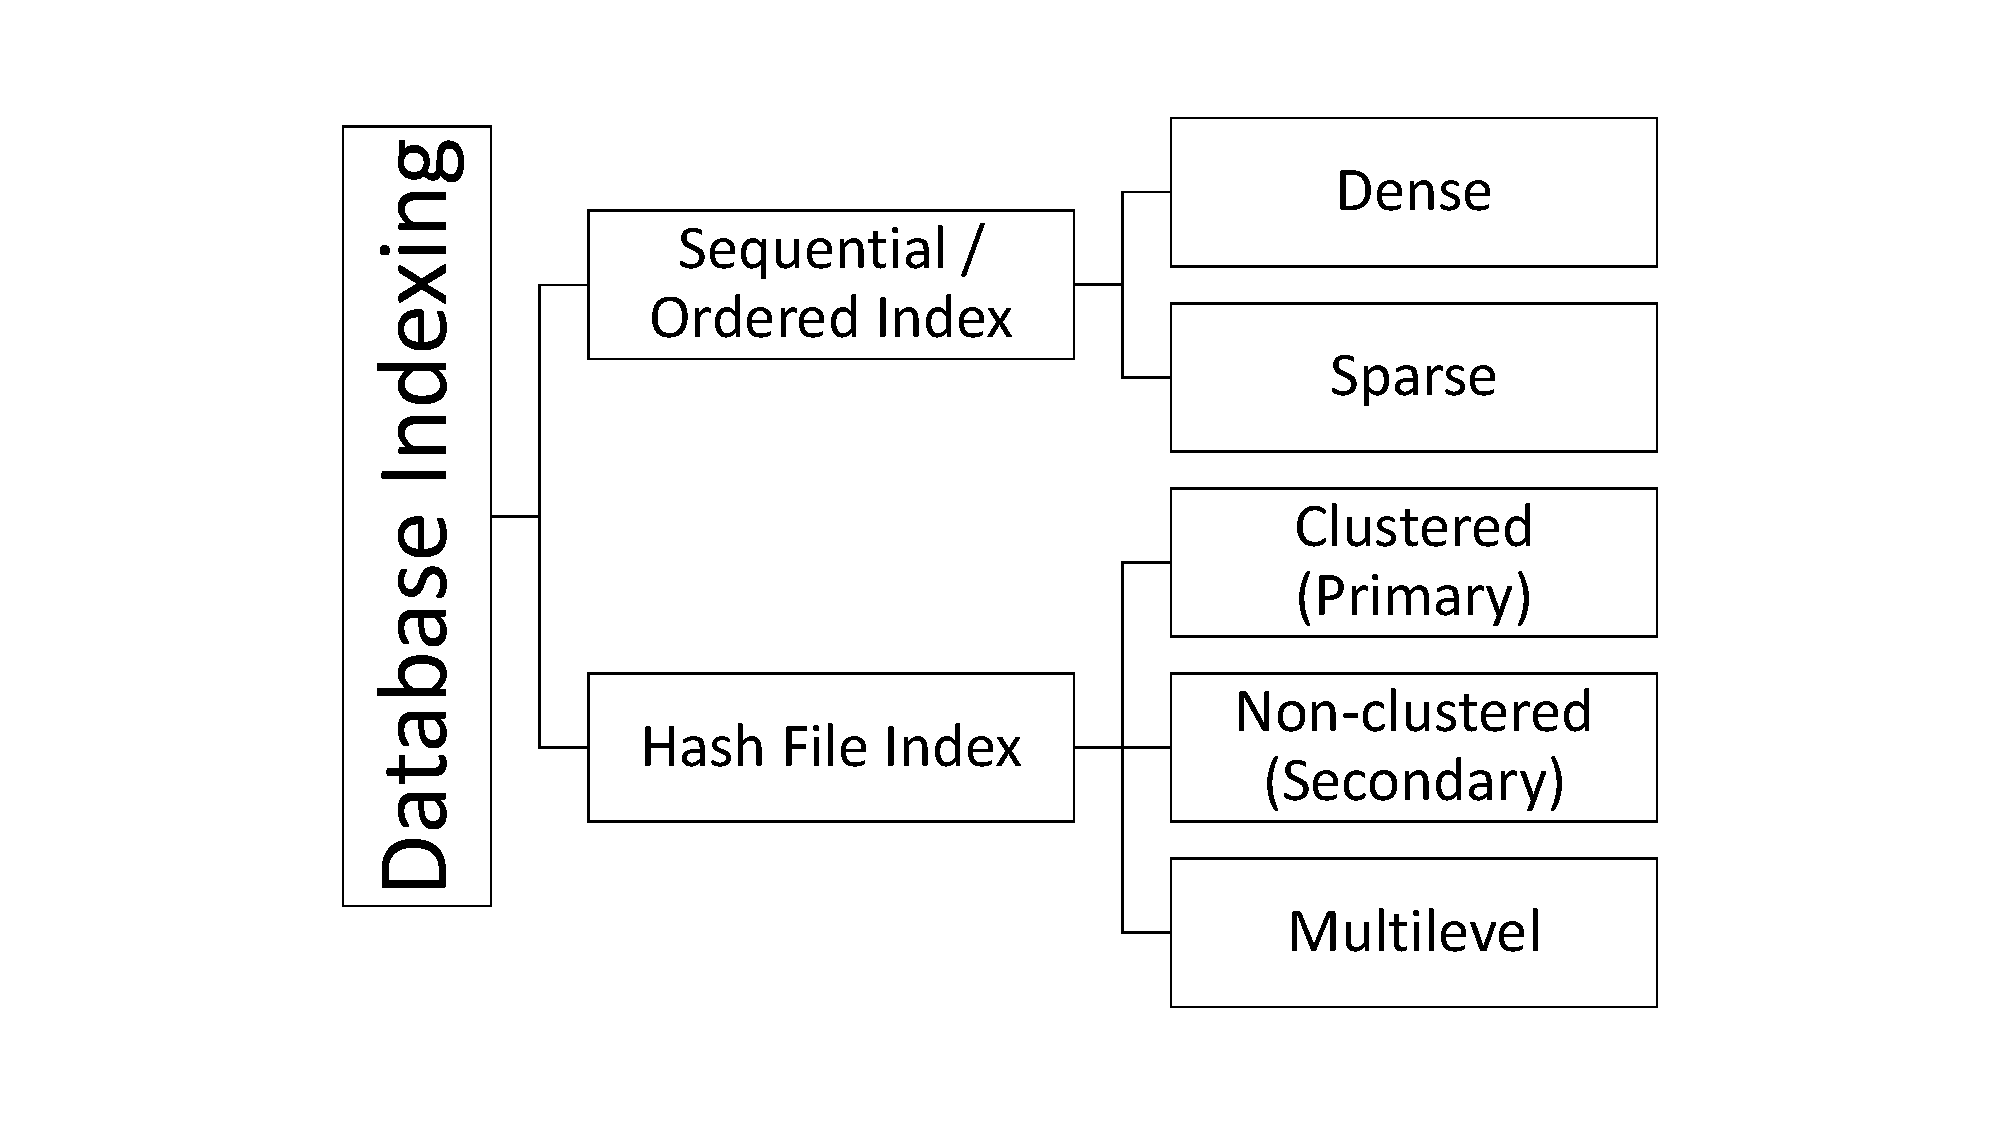
\includegraphics[width=0.55\textwidth]{images/Classification of database indexing.pdf}
    \caption{Classification of Database Indexing \cite{garcia2008database}}
    \label{fig:index_class}
\end{figure}

\subsubsection{Indexing of Biometric data}
Almost all applications of biometric systems involve dealing with large amounts of complex data which can be in the order of millions. 
Also, biometric data never follows any natural sorting order, because of which traditional/database indexing mechanisms do not work well for biometric systems. 
One of the major limitations of the existing biometric systems is query matching for large databases which often causes inefficient data retrieval. 

Traditional indexing techniques like k-d tree-based indexing, geometric hashing, k-means clustering, etc. index the records in alphabetical or numeric
order. These traditional algorithms have been used with multi-dimensional
data, but, they fail with multidimensional biometric data as it is non-correlated. More importantly, biometric data has a huge variety of features, thus, it is important to
consider unique identifiers which are more resilient to distortion and provide better
accuracy even with the presence of noise.

This work proposes a novel indexing scheme for retrieving biometric data using features extracted from a single biometric trait as well as from multiple biometric traits. Going by the block diagram of a generic biometric system given in Figure \ref{fig:bio_sys_block}, this work focuses on \textit{Data Storage} and \textit{Signal Processing} subsystems. At first, uni-modal biometric features are considered for indexing. Afterward, a multi-modal indexing approach has been proposed by taking into consideration more than one biometric trait. Several challenges
posed by the biometric traits, such as distortion due to scaling and rotation, need to be resolved in order to achieve the best results from the index. 

% \subsection{Cryptograpic Keys}

% Cryptographic keys generated using hardware or software pseudo-random generators
% are arduous to maintain. Such keys need to be stored or should be with a reduced
% length so that they can be remembered, neither of which is secure. Storing the
% keys make them susceptible to theft or adversarial attacks, whereas short keys
% are prone to dictionary attack. With the rapid advancement of cryptographic
% applications, IoT applications, etc.~\cite{alassaf2019enhancing,
% 	panchal2018novel}, the need to ensure system security along with increased
% system usability is more than ever.  This work addresses the above concerns
% and proposes a novel approach to key generation from a user's biometric data.
% With the great success of biometric data in the domains of personal identification
% and verification, researchers are now focusing on crypto-biometric
% systems~\cite{barman2015security, panchal2018novel}. Crypto-biometric systems are
% a combination of biometric authentication with cryptographic promise to provide
% a solution to the existing security problems \cite{schultz2018biometric,
% 	panchal2020designing}. These authentication systems have
% 	used fuzzy vault or fuzzy commitment~\cite{yang2014delaunay}, also known as
% 	static authentication.
%     \par


% In order to address the problem of static authentication, a
% 	novel cryptographic key generation technique is proposed in this work. The
% 	proposed scheme generates a dynamic key from a fingerprint using hybrid
% 	features such as minutia points and texture-based information. The dynamic
% 	nature of the key depicts that there is no need to store the original key or
% 	biometric template itself.  Furthermore, the relative feature vector derived
% 	from DTN does not reveal the minutia point information. Moreover, the hybrid
% 	feature vector increases the performance accuracy by addressing the
% 	limitations of only considering a single feature.
    
% 	\par
